\documentclass[a4paper,11pt]{article}

\usepackage{times} 
\usepackage{graphicx}
\usepackage{datetime}
\newdateformat{monthyeardate}{%
  \monthname[\THEMONTH], \THEYEAR}
\usepackage{tikz}
\usepackage{blindtext}
\usepackage{pgfplots}
  
\newcommand{\report}{TBD}
\newcommand{\name}{Marius Marmakas}

\begin{document}
\begin{titlepage}
  \centering
    \vfill
    
\includegraphics[width=8cm]{vulogo.png} %also works with logo.pdf
    \vfill
    {\bfseries\Large\course\vskip2cm}
    {\bfseries\LARGE\report\vskip2cm}
    {\Large\name\vskip2cm
      Department of Computer Science\\
      Vrije Universiteit Amsterdam\\
      \vskip2cm
      \monthyeardate\today\\}  
    \vfill
\end{titlepage}
\newpage
\tableofcontents
\newpage

\title{\report}
\author{\name}
\date{}
\maketitle

% Start your sections here
\section{Introduction}
\indent TBD is a take on the classic Killing Floor series. One of the common complaints about the latest Killing Floor entry is limited support for multiplayer lobbies. At the cost of reduced graphics, TBD aims to showcase an elegant take on multiplayer game networking via Python. TBD mixes the genre formula by adding new elements of play to the content of the game to create a different experience - a balance between player interaction and pattern discovery, accompanied by responsive movement and 2D artwork.
\subsection{How To Play}
\begin{itemize}
    \item The game consists of 3 stages, each contains a subset of levels. Number of levels in the stage increases exponentially, each level start preparation phase. This is the best time to gear up, because as the amount of levels increases, so does the amount of time needed to survive.
    \item Gear, Tools and Weapons may drop from monsters, its quality depends on the monster, current progress and player performance, as later on discussed in System Design. Most patterns inside of the game will usually contain any combination of these conditions.
    \item Moreover, be sure to check out the ability tab. You can spend experience points gained from fighting monsters to exchange it for useful techniques, which may help later in the game. Good luck!
\end{itemize}
\section{System Design}
\indent The system of TBD is designed to intuitively teach the person playing how to tackle a new problem or pattern. The teaching is realized through a rule-set, tailored to be flexible and dynamic to allow all play styles and encourage learning. A rule-set can be viewed as a graph, where vertices are requirements and edges are the connection between requirements. By interconnecting vertices in rule-set graph, I increase the number of paths the player can take, therefore providing multiple opportunities for the player to learn and increasing content \textbf{insert formula}. A pattern is a series of requirements the player chooses to play by. A couple examples of a requirement are: "all good potions have a high color hue" and "shiniest items are the most cheap". A dynamic, interconnected rule set will be further described in the section Requirements.\\
\indent Additionally, system rewards or punishes the players based on their performance, not on their play style. Were a group of players punished for using a certain play style, they would all quit the game, because the game can no longer teach it's patterns, effectively denying its users. At the very least, the TBD system tries to avoid limiting the user experience by carefully selecting the requirements.
\section{Requirements}
Requirements within the TBD make up an interconnected system. The requirements are divided into items, hereinafter all requirement descriptions start with the word "Should".
\begin{itemize}
    \item Art
    \begin{enumerate}
        \item Should adhere to the cosmos-horror theme.
        \item Should use either 16x16 or 32x32 pixel canvas.
        \item Should portray a clear representation of an object.
        \item Should reuse abilities and their animations by shifting the hue.
        \item Should utilize impressionistic play of light on objects, that require attention.
        \item Should contrast objects to the background from the view of an object (e.g., a gun contrasts the player and player contrasts the background).
    \end{enumerate}
    \item Animations
    \begin{enumerate}
        \item Should be less or equal 8 frames for all effect.
        \item Should be less or equal 4 frames for all movement.
        \item Should result in a smooth procedural flow when played back.
    \end{enumerate}
    \item Players
    \begin{enumerate}
        \item Should drop items on death.
        \item Should contain an animation set.
        \item Should be able to damage other players.
        \item Should re-spawn in the proceeding level.
        \item Should retain experience points on death.
        \item Should be able to accumulate experience points.
        \item Should be able to equip and use items, gear, abilities.
        \item Should be able to spend experience points to unlock abilities.
    \end{enumerate}
    \item Monsters
    \begin{enumerate}
        \item Should contain an animation set.
        \item Should target the nearest player.
        \item Should drop experience points and varied quality items.
        \item Should scale in skill level reflective of the game progress.
        \item Should interchange skills with other type of monster every level.
        \item Should artistically represent at least one socially recognized fear.
        \item Should have at least a couple of interchangeable skills, independent of monster type.
    \end{enumerate}
    \item Objects
    \begin{enumerate}
        \item Should display visual cues when used.
        \item Should contain an animation set if applicable.
    \end{enumerate}
    \item System
    \begin{enumerate}
        \item Should display subtitles for new events.
        \item Should display a concurrent lobby listing.
        \item Should allow players to create their own lobbies.
        \item Should display personal and lobby player statistics.
        \item Should adhere the game difficulty to the progression graph in Figure \ref{fig:progress-graph}.
    \end{enumerate}
\end{itemize}
\begin{figure}
    \centering
    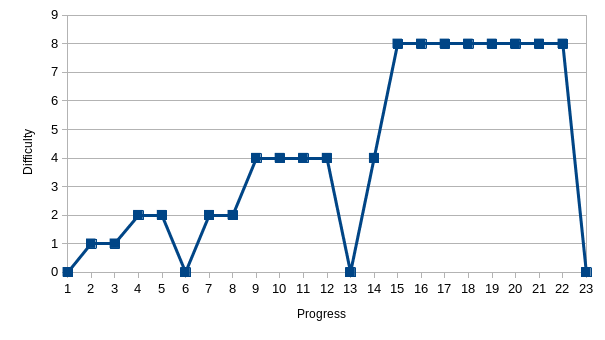
\includegraphics[scale=0.5]{images/progress-graph.png}
    \caption{TBD Level Progress}
    \label{fig:progress-graph}
\end{figure}

\end{document}
% End your sections here

\bibliography{refs}
\bibliographystyle{plain}

\end{document}
